%%%%%%%%%%%%%%%%%%%%%%%%%%%%%%%%%%%%%%%%%%%%%%%%%%%%%%%%%%%%%%%%%%%%%%%%%%%%
% AGUtmpl.tex: this template file is for articles formatted with LaTeX2e,
% Modified March 2013
%
% This template includes commands and instructions
% given in the order necessary to produce a final output that will
% satisfy AGU requirements.
%
% PLEASE DO NOT USE YOUR OWN MACROS
% DO NOT USE \newcommand, \renewcommand, or \def.
%
% FOR FIGURES, DO NOT USE \psfrag or \subfigure.
%
%%%%%%%%%%%%%%%%%%%%%%%%%%%%%%%%%%%%%%%%%%%%%%%%%%%%%%%%%%%%%%%%%%%%%%%%%%%%
%
% All questions should be e-mailed to latexagu.org.
%
%%%%%%%%%%%%%%%%%%%%%%%%%%%%%%%%%%%%%%%%%%%%%%%%%%%%%%%%%%%%%%%%%%%%%%%%%%%%
%
% Step 1: Set the \documentclass
%
% There are two options for article format: two column (default)
% and draft.
%
% PLEASE USE THE DRAFT OPTION TO SUBMIT YOUR PAPERS.
% The draft option produces double spaced output.
%
% Choose the journal abbreviation for the journal you are
% submitting to:

% jgrga JOURNAL OF GEOPHYSICAL RESEARCH
% gbc   GLOBAL BIOCHEMICAL CYCLES
% grl   GEOPHYSICAL RESEARCH LETTERS
% pal   PALEOCEANOGRAPHY
% ras   RADIO SCIENCE
% rog   REVIEWS OF GEOPHYSICS
% tec   TECTONICS
% wrr   WATER RESOURCES RESEARCH
% gc    GEOCHEMISTRY, GEOPHYSICS, GEOSYSTEMS
% sw    SPACE WEATHER
% ms    JAMES
% ef    EARTH'S FUTURE
%
%
%
% (If you are submitting to a journal other than jgrga,
% substitute the initials of the journal for "jgrga" below.)


\documentclass[linenumbers]{agujournal2018}
%\usepackage{apacite} %PMC not sure who changed natbib to apacite, but it broke all of my citations...
\usepackage{natbib}
\usepackage{url} %this package should fix any errors with URLs in refs.
\usepackage{verbatim}
%\usepackage{hyperref}
%\hypersetup{citecolor=black}
%\usepackage{subcaption}
%\usepackage{subfig}
\usepackage{amsmath}


%\documentclass[draft,ms]{AGUTeX}
%\usepackage{graphicx}
%\usepackage[modulo]{lineno}

\usepackage[%
  color=gray
 ,scale=20
 ,placement=top
]{background}

\backgroundsetup{contents={DRAFT}}

% Set to \draftfalse and it spaces lines for the journal, \draftrue compresses it for fewer printed pages
\drafttrue

%% Shortcuts %%
\def\deg{$^\circ$}


%-------------------------------
%  Main Text from tex sub files
%-------------------------------

%% WORDS %%
%1495 OCT 23
\journalname{Journal of Advances in Modeling Earth Systems (JAMES)}
\begin{document}

\title{The NCAR Community Atmosphere Model, version 6 (CAM6): Scientific Configuration and Simulation Fidelity}

%% ------------------------------------------------------------------------ %%
%
%  AUTHORS AND AFFILIATIONS
%
%% ------------------------------------------------------------------------ %%


%Use \author{\altaffilmark{}} and \altaffiltext{}

% \altaffilmark will produce footnote;
% matching \altaffiltext will appear at bottom of page.


 \authors{
R. B. Neale\affil{1}, 
J. Bacmeister\affil{1},
C. Hannay \affil{1}, 
A. Gettelman\affil{1},
P Bogenschutz \affil{2},
H. Morrison\affil{1}, 
X. Liu \affil{3},
C. Bardeen \affil{1},
V. E. Larson\affil{4}, 
P. Lauritzen \affil{1},
M. Zhang\affil{5},
M. A. Taylor\affil{6},
C. Jablonowski\affil{7},
P. M. Caldwell\affil{2}
}

\affiliation{1}{National Center for Atmospheric Research (NCAR), Boulder, Colorado, USA.}
\affiliation{2}{Lawrence Livermore National Laboratory, Berkeley, California, USA}
\affiliation{3}{Department of Atmospheric Science, University of Wyoming, Wyoming, USA.}
\affiliation{4}{Department of Mathematical Sciences University of Wisconsin, Milwaukee, Wisconsin}
\affiliation{5}{School of Marine and Atmospheric Sciences, Stony Brook University, Stony Brook, New York}
\affiliation{6}{Sandia National Laboratories, Albuquerque, New Mexico}
\affiliation{7}{Department of Climate and Space Sciences and Engineering, University of Michigan, Ann Arbor, Michigan}

\correspondingauthor{Richard Neale}{rneale@ucar.edu}

\linenumbers
\modulolinenumbers[1]

\begin{abstract}

The NCAR/DOE Community Atmosphere Model, version 6 (CAM6) is the atmosphere component of the Community Earth System Model, version 2 (CESM2). It is a significant advance from previous model versions, in the representation of physical procesess and simulation performance. With the exception of the deep convection parameterization, all macroscale cloud processes and dry turbulence parameterizations have been replaced by the Cloud Layers Unified By Binormals (CLUBB) unified moist turbulence scheme. It simulates co-occurring turbulence regimes, including clouds, dry convective and stably stratified regimes. Its major advantage is a continuous representation of many physical processes that were previously represented in conceptually separate parameterizations. 

Microphysical processes are now represented by an updated version of the Morrison-Gettelman (MG2) microphysics that includes predicted mass and number concentrations of rain and snow. Aerosol processes include an additional mode as part of the Modal Aerosol Scheme (MAM4) the additional mode is able to more accurately represent black carbon chemical processes.  New surface drag parameterization and gravity wave schemes have been significantly updated to include stress tendencies that now impact above the lowest model level, and anisotropic sub-grid orographic for wave emission.

The performance in AMIP simulations surpasses that of CAM5 for many mean climate features including precipitation, humidity and critically short-wave cloud forcings that are integral to the increased climate sensitivity of CESM2. Regionally CLUBB thermodynamic tendencies match the sum of the equivalent processes that are represented separately in CAM5. The caveat to this is that there is clearly compensation for the deep convection, which is reduced and consequently results in a convective precipitation fraction lower than CAM5, which is considered more realistic. The performance compared to CAM5 is marginal, but in the coupled model it's significant and results from MAM and DJF improvements of poor performance in CESM1, especially as it relates to tropical Pacific surface stresses and rainfall.



An analysis of sensitivity experiments reveals that precipitation skill improvements are, to a certain extent, attributable to increases in deep convection sensitivity during Winter. However more complicated causes emerge in Summertime where tuning parameters changed during model development would seem to be equally as important. In actual fact, interim tuning parameters used in coupled model development deliver a better climate than the release version of CAM6.

Significant performance degradation is, however, seen in the large-scale flow. Increased tropospheric biases reflect an erroneous poleward shift in the westerly jets, and this can be attributed to the shift to CLUBB and improvements to the microphysics parameterization.

\end{abstract}
\pagebreak
\section{Introduction}
\label{sec:intro}

The National Center for Atmospheric Research (NCAR) Community Atmosphere Model, version 6 (CAM6) is the atmospheric component of the Community Earth System Model, version 2 \cite[CESM2,][]{Danabasoglu2020}. CAM6 was a collaborative development effort between NCAR, partner universities and national labs and is a significant enhancement to the representation of atmospheric processes compared to CAM5 \citep[][]{Neale2012}. Its development targeted existing missing and incomplete processes, and in particular those key to cloud feedbacks \citep{Webb2017}, cloud aerosol interactions \citep{Stevens2015} and climate sensitivity \citep{Zelinka2020}. Consequently cloud processes were the primary focus of the development effort. Historically, parameterizations of cloud processes have been compartmentalized into different approximations of closely related phenomena, namely shallow convection, boundary layer processes and resolved-scale condensation, each employing different approximations. However, this is artificial and is subject to non-commutative process ordering properties \citep{Donahue2018}, in addition to poor scale-aware properties. In CAM6 a partial unification has been implemented with the Cloud Layers Unified By Binormals \citep{Golaz2002,Golaz2002a} scheme, under the umbrella paradigm of high-order moist turbulence. Microphysics, surface stress, vertically propagating gravity waves and aerosol parameterizations further advance the suite of physical processes from CAM5. The combination of these processes have combined to produce climate forcings, and feedbacks significantly different to CAM5 \citep{Gettelman2019}. Understanding these interactions is crucial, given the extensive contributions from CESM2 and CAM6 to the current Coupled Model Intercomparison Project \citep[CMIP6, ][]{Eyring2016a}.

The purpose of this paper is three fold. To document the scientific configuration of CAM6 and analyze changes in the climate features compared to previous model versions. The representation of coupled dynamical large-scale modes of variability \citep{Simpson2020}, and versions of the model with an elevated model top \cite{Gettelman2019} are mostly favorable compared to CAM5. By analyzing AMIP configurations of CAM5 and additionally CAM4 \citep{Neale2013} here, the focus will be on any monotonicity in the recent trajectory of model skill. Meaning, can improvements during this cycle of development be identified as a trend or as a recovery of degradation seen in the preceding model cycle. 

To summarize the regional equilibrium of parameterized processes. In particular, given the more general moniker of moist turbulence in CAM6, is it possible to diagnose the climate regimes in a similar to CAM5 where state tendencies are assigned explicitly to its compartmentalized parameterizations. To attribute net climate differences in CAM6 to incremental physics changes applied as part of the development process. Given the significant modification to cloud feedbacks seen in CAM6 \citep{Gettelman2019} and the resultant increase in the benchmark equilibrium climate sensitivity, from 4.2K to 5.3K, in CESM2 with largely the same ocean component as CESM1 \citep{Bacmeister2020}, it is critical to understand these changes. Importantly, the physics changes are not uniquely selections of parameterization choices between CAM5 and CAM6, but also tuning parameters which frequently have impacts as large as an individual parameterization choice. Unlike previous model versions CESM2 was developed mostly in a fully coupled framework. Indeed, it's worth noting that a good deal of effort in tuning went not into tuning the atmosphere itself, but into tuning the whole of the coupled system. Because of this approach the true sensitivities of the CAM6 climate, to parameterization choice and settings are not well understood in an AMIP framework, and so this analysis aims to understand these further.


The analysis in this paper strives to address performance in the climate simulation when placed against the backdrop of previous model versions, parameterization selection, and parameter sensitivities. Section \ref{sec:description} outlines the major parameterization changes, with a comparison of simulated climate in Section \ref{sec:climate}. A more in depth analysis of CLUBB is provided in Section \ref{sec:tendencies} and an explorations of many of the important parameter and parameterization sensitivities in CAM6 is shown in Section \ref{sec:sensitivities}. Finally, summary and conclusion in Section \ref{sec:conclusions}.


\section{Scientific Configuration}
\label{sec:description}
Fundamental changes in the representation of physical processes were made for CAM6. These include complete replacements of boundary layer turbulence, shallow convection, cloud macrophysics, and surface stress due to sub-grid scale orography parameterizations. In addition, significant changes were made to the cloud microphysics, aerosol physics and deep convection. Also, of note are the values of calibration or tuning parameters of parameterization schemes that remain from CAM5. They are not considered a modification to parameterizations themselves here, but many take different values to CAM5 mostly in an effort to produce skillful improvements in the CAM6 climate. The individual roles of these parameterization and tuning changes are examined in Section \ref{sec:sensitivities}. Of the primary physics parameterizations only the Rapid Radiative Transfer Scheme for GCMs \citep[RRTMG,][]{Iacono2008,Mlawer1997} remains largely unchanged. 

\subsection{Cloud Macrophysics and Turbulence}

Shallow convection \citep{Bretherton2004}, planetary boundary layer \citep{Bretherton2009} and cloud macrophysics \citep{Park2014} schemes in CAM5 are replaced with a new unified turbulence scheme, the Cloud Layers Unified By Binormals \citep[CLUBB,][]{Golaz2002a,Golaz2002}. CLUBB determines these processes as part of higher order solutions to the 3D turbulence equation. Where, for example, vertical velocity variance $w'^{2}$ evolution is given by:

%
\begin{eqnarray}
  \frac{\partial\overline{w'^2}}{\partial 
t}=-\overline{w}\frac{\partial\overline{w'^2}}{\partial z}-\frac{\partial\overline{w'^3}}{\partial z}-2\overline{w'^2} \frac{\partial\overline{w}}{\partial z}+\frac{2g}{\theta_0}\overline{w'\theta_v'}-\frac{2}{\rho}\overline{w'\frac{\partial p}{\partial z}}-\epsilon_{ww}
\end{eqnarray}

with second order source terms of vertical advection, third order gradients, gradient mean advection, buoyancy generation, pressure related terms and dissipation.

Solutions are achieved by describing vertical velocity, $w$, liquid water potential temperature, $\theta_l$ and total specific water content $q_t$ within
assumed joint Probability Distribution Functions (PDFs) 

\begin{eqnarray}
  \overline{{w'}\,{\theta_l'^m}\,{ q_t'^n}}  =  \int\int\int(w-\overline{w})^l(\theta_l-\overline{\theta_l})^m(q_t-\overline{q_r})^n P(w,\theta_l,q_t)\,dw\,d\theta_l\,dq_t
\end{eqnarray}

 and in this implementation are specifically characterized by two Gaussian PDFs. They provide a self consistent description of mean and higher order quantities in moist turbulent properties. A previously implemented configuration in a pre-cursor to CAM \citep[CAM5.5, ][]{Bogenschutz2018} has been shown to represent effectively the skewness in properties associated with deeper convection, as in \citep{Bogenschutz2010}. In comparison to the separate schemes of CAM5 the calculations for liquid cloud fraction, total liquid, variance and eddy flux variances are self consistent.



\subsection{Microphysics}
\subsubsection{Liquid Processes}

Cloud microphysics uses version 2 of the \cite{Morrison08} scheme, described by \cite{Gettelman2015} and with model performance shown in \cite{Gettelman2015a}. The Major change is that precipitation species are now handled in a prognostic rather than diagnostic manner. Mass and number concentrations of ice (snow) and liquid (rain) are thus determined from the following budget approximations:

\begin{eqnarray}
  \frac{\partial q_x}{\partial t} & = & -\frac{1}{\rho}\nabla\dot(\rho \mathbf{u} q_x) - \frac{1}{\rho}\frac{\partial(\rho V_{q_x}q_x)}{\partial z}+S_{q_x}  \\
  \frac{\partial N_x}{\partial t} & = & -\frac{1}{\rho}\nabla\dot(\rho \mathbf{u} N_x) - \frac{1}{\rho}\frac{\partial(\rho V_{N_x}N_x)}{\partial z}+S_{N_x}
\end{eqnarray}
where $q_x$ and $N_x$ are the mean and number concentration of species $x$ respectively. 

CLUBB is sub-stepped within the microphysics in order to maintain stability within the parent full physics timestep of 30 minutes, a period much longer than for which the scheme was developed \citep{Golaz2002}. It is further required to avoid spurious oscillations seen previously \citep{Zheng2017}  Substepping can vary, but in the default configuration there are three instantiations of CLUBB per MG2 call, and one MG call per physics timestep.

\subsubsection{Ice Processes}

A number of changes have been made to the cloud microphysics for CAM6 to improve water vapor and ice clouds in the Upper Troposphere and Lower Stratosphere (UTLS) including: adding subgrid variability for ice growth, changing the minimum ice particle size, adjusting the fall velocity for small ice particles, and making corrections to ice nucleation. The most important of these changes is supporting subgrid variability by the addition of a scaling factor ($Q_{sfac}$) to the water vapor saturation required for cirrus growth. In CAM5, the ice cloud fraction began at a relative humidity threshold ($RH_{mini}$) of 0.8; however, the threshold for cloud growth was ice saturation (1.0). This inconsistency caused too little moisture to be condensed in the tropics by the cold trap resulting in too much water vapor entering the stratosphere. In CAM6, scaling the saturation threshold by $Q_{sfac}$ allows condensation growth to occur in part of the gridbox starting at $RH_{mini}$, improving stratospheric water vapor. To support smaller ice particles in the UTLS, the minimum ice particle size has been decreased from a diameter of 10 $\mu$m to 1 $\mu$m and the fall velocity has been adjusted assuming that small particles ($<$ 36 $\mu$m) have a bulk ice density, rather than the reduced density used for larger ice particles. Finally, several changes have been made to improve ice nucleation including: correcting the calculation of the number of dust ice nuclei (IN), moving heterogeneous IN from interstitial to cloud-borne aerosol following nucleation, and using the gridbox average relative humidity for homogeneous freezing rather than assuming all homogeneous freezing is in-cloud with a relative humidity of 1.0. Some initial support has been provided for Type II (ice) polar stratospheric clouds by allowing different cloud settings in the stratosphere and including homogeneous freezing of accumulation and coarse mode sulfate particles in the stratosphere. These changes are described in more detail in Bardeen et al. (2017).

\subsection{Deep Convection}
CAM6 retains the vast majority of the \cite{Zhang1995} configuration for the representation of deep convection processes.  The settings that control ZM are however used as major tuning parameters that optimize the climate produced in CAM6 and more importantly coupled versions of CESM2. The optimizations are primarily for the global radiative balance of the climate, in particular the cloud radiative components, and also for precipitation distributions. The parameters include the autoconversion and evaporation of falling precipitation efficiencies and the strength of convective momentum transports. As is apparent in section \ref{sec:sensitivities}, changes in these parameters can have impacts on atmospheric climate that are comparable with the introduction of new process parameterization.

\subsection{Sub-grid Surface Drag}
An update surface drag scheme based on \cite{Beljaars2004} replaces the simple Turbulent Mountain Stress \cite[TMS, ][]{Richter2010} scheme which simulated an effective near-surface drag, due to sub-grid scale variations of orographic roughness. Whereas TMS was applied to the lowest model level only, \cite{Beljaars2004} is applied over a number of levels based on a spectral integral of the impact of orographic heights, represented as an exponential height decay in the stress
\begin{eqnarray}
  F_x=-\alpha\beta C_{md} C_{corr}|U(z)|U(z)2.109e^{-(z/1500)^{1.5}}a_2z^{-1.2}, 
\end{eqnarray}

\subsection{Aerosols}
The modal aerosol model representation is retained for CAM6. The 3-mode implementation from CAM5 \citep[MAM3, ][]{Liu2012} is augmented with an additional mode representation \citep{Liu2016}. This accounts explicitly for the microphysical ageing of primary carbonaceous aerosols in the atmosphere. Specifically the extra mode accounts for primary organic matter (POM), black carbon (BC) and there associated number characteristics. The mode properties interact with the existing accumulations mode through condensation an coagulation. In isolation this change is able to increase the concentration of organic matter by 40\% remote from major source regions \citep{Liu2016}. Polar regions in particular see a beneficial increase in burdens particular in the colder seasons. However, these improvements exist against the background of circulation dependent biases seen in previous versions of CAM with MAM3 \citep{Ma2013}.

Specific to the representation of dust, between CAM5 and CAM6 there was a switch in the mode size parameters for the coarse mode (mode 3).  In order to improve the performance of the stratospheric aerosols, the sigma (width of the coarse mode) as decreased from 1.8 to 1.2. In addition, the edges of the coarse mode were moved to be more limited, and the number mean diameter was moved  from 2.0 to 0.9. These changes impact the properties of the coarse mode aerosols in the troposphere as well (Li et al., in prep.,10.5194/acp-2020-547 ).  The dust and sea salt direct radiative interactions are more negative by ~-0.40W/m2 for both aerosols, because of the smaller size assumed for the aerosols for some interactions (Li et al., in prep. 10.5194/acp-2020-547).

\subsection{Additional Developments and Relevant Changes}

Formulation of the spectrum of orographically generated waves continues to follow the scheme of \citep{McFarlane1987}. In CAM6 it uses information using ridge orientation derived from the underlying orographic dataset. This now determines the orientation of the applied drag force. The use of ridge height estimates also allows the application of form drag following the methodology of \cite{Scinocca2000}, which can account for high drag situations e.g., during down slope wind events.

\subsection{Dynamical Core and Resolution}
Although, CAM6 retains the hydrostatic, finite volume \citep{Lin1996,Lin2004} dynamical core with a resolution close to 1$^\circ$, an option for the spectral element dynamical core is now available \citep{Lauritzen2018}, but has not bee analyzed here. A modest increase in the vertical resolution from 30 to 32 levels has been applied, but these levels are in the upper troposphere and designed to exactly coincide with WACCM6 level locations in order to provide similar resolutions for the string vertical gradients and equally represent specific processes that at least begin there, such as the tape recorder effect. And allow simultaneous climate tuning \citep{Gettelman2019}.

\subsection{Datasets}
Of known impact on recent CAM simulations is the transition from a simple interpolation of the USGS 30-second digital orographic height dataset \citep[GTOPO30,][]{Gesch1999} to the Global multi-resolution terrain elevation data 2010 \citep[GMTED2010,][]{Danielson2011} and using a more spectrally consistent generation of mean and height variances \citep{Lauritzen2015} used as boundary forcing in the gravity wave drag and surface stress \citep{Beljaars2004} parameterizations. The core set of forcing data also changes from the CMIP5 \citep{Lamarque2010} recommended source to the CMIP6 source \citep{Feng2020}. A notable change is that a number of datasets with decadal time frequency now have annual frequency in CMIP6, as well as seasonal detail added to annual variables.

\subsection{Model Tuning Parameters}
Tuning parameters can often influence the climate performance of a GCM to the same extent as core parameterization choices. In particular they are used as calibration or 'tuning' tools to produce a energetically consistent climate for climate change studies. A common practice for CESM and many other models \citep{Schmidt2017} is to produce a net zero energy budget (combined long wave and short wave radiation components) at the top of the model atmosphere domain or at the lid, as the default version of the model \citep{Danabasoglu2020}.

-GHG dataset

-Sea salt bins
-Deposition
-CLUBB liquid supersat problems.
-Ozone chem (obs versus WACCM)
-Background volcanics
-CLM4.5?

-Sea spray (salt and organics) do not contribute to INP and also organics are not included
-Organics are being put int E3SM
\section{Mean Climate Skill}
\label{sec:climate}

There have been significant simulation improvements in CAM6 relative to CAM5. Many of these can be attributed to changes in individual physical process, but a number have occurred due to the calibration or 'tuning' carried out in the context of a fully coupled version of CESM2. The Normalized Mean Standard Error (NMSE) shown in Fig. \ref{f_CAM_CESM_NMSE_DJF_JJA} summarizes error statistics, including bias and phase errors, for the northern hemisphere seasonal 200-mb height fields. The legacy of models back to CAM3 \citep{Collins2006} generally shows December/January/February (DJF) errors to be smaller when SSTs are prescribed (AMIP), versus when an active ocean model is used. CAM6 departs from this behavior as the CESM2 error is of comparable magnitude, reflecting the focus shift in the model development cycle, between AMIP and coupled. Although the CESM2 unconditional bias is reduced by a factor of four from CESM1, changes over time have been monotonic. A significant degradation from both CCSM3 \citep{Collins2006} and CCSM4 \citep{Gent2011} to CESM1 exists, and reflects a cool late 20th century climate, as well as cyclonic biases over the ocean basins. 

Errors in DJF are generally determined by variations in the oceanic storm track climate, a well simulated phenomenon in climate models. In June/July/August (JJA), however, errors are characterized by large scale monsoonal circulations and rely on more poorly constrained land-atmosphere coupling \citep{Dirmeyer2006}, hence the higher overall NMSE. Although CESM2 errors indicate it is the most skillful coupled model, the CAM6 AMIP simulations do not perform nearly as well as even CAM4. Given the non-negligible SST biases in CESM2 \citep{Danabasoglu2020}, one could infer that CESM2 performs better for the wrong reasons, which will become apparent in later analyses. Errors for all model configurations easily exceed differences among different analyses products by a factor of ten in DJF and a factor of five in JJA. The trend in NCAR model development indicates that CCSM4 may be a more skillful model than CESM1, and for this reason we also consider the performance of CCSM4 in what follows.

A broader summary of the change in model skill is shown through Taylor Diagrams \citep[Fig.\ref{f_TAYLOR_CAM_CESM},][]{Taylor2001} for both AMIP and coupled versions using CESM. Systematic improvements in the most challenging climate fields (such as precipitation and cloud forcing fields) are only marginally apparent in AMIP simulations. Correlation of precipitation fields improve by almost 0.1 between CAM5 and CAM6, but this comes at the cost of degradation in the seasonal, temporal and spatial variance (standard deviation) over land. It is recognised that different versions of the community land model (CLM) can also influence this pattern  The coupled simulations contrast markedly with AMIP, since the less skillful fields (including Pacific zonal surface stress) are systematically improved between CAM4 and CAM6. Cloud radiation fields improve markedly, the regional changes of which are highlighted below. While the scaled RMSE improves to 0.82 in CESM2, the mean bias has improved only after a significant degradation in CESM1 and CAM5 (similar to above) and that was primarily related to more poorly simulated long wave cloud forcing and ocean precipitation in this model version.

The regional precipitation distribution is significantly improved in CAM6; decreasing RMSE by more than 10$\%$, but Indo-Pacific biases still continue to dominate (Fig. \ref{f_PRECT_2D_CAM456}). Over the Western Indian Ocean and Arabia wet biases have been mostly illuminated, decreasing from in excess of 3 $mm/day$ and corresponding to an excess of 100$\%$ of the observed values. Seasonally, this reduction occurs in the pre-monsoon period, and is reflective of CLUBB effectively capping cloud depth within the southerly and south-westerly flow region REF??. The Inter Tropical Convergence Zone (ITCZ) remains a persistent problem in CMIP models \citep{Tian2020} and CAM is no exception, with persistence in ITCZ errors through previous model versions. The Pacific ITCZ bias is virtually illuminated in CAM6, the source of which will be discussed in section \ref{sec:sensitivities}. In contrast to this is the Atlantic ITCZ where precipitation amounts are now lower than 25\% of observed.

In the seasonal zonal mean distribution (Fig. \ref{f_PRECT_1D_DJF_CAM456}), there are clear improvements seen in DJF and most obviously related to a 50\% reduction from the East Pacific ITCZ. This is not reflected in coupled CESM2, where wet biases reside mostly to the South of the equator. Similarly in CESM1 and CCSM4, where AMIP biases tend to be small, the coupled bias are largest. In JJA (Fig. \ref{f_PRECT_1D_JJA_CAM456}) the relationship between the East Pacific ITCZ biases in AMIP and coupled models changes compared to DJF. Coupled CESM2 wet biases are larger than 2 $mm/day$ where CAM6 is dryer than observed. Contrasting coupled versus AMIP precipitation biases serves to emphasize the locking of the precipitation to the prescribed SSTs in all model versions, but with greater variations seen in the bias pattern of coupled configurations.

Although the ITCZ bias is largely remedied in DJF it does not accompany decreased biases in the upper tropospheric flow. The 200-mb rotational and divergent circulation (Fig. \ref{f_PSICHI_2D_DJF_CAM456_diff}), which are markers of the large-scale response to tropical convective heating, imply an anomalous increase in the CAM6 convective outflow compared to CAM5, when biases were minimal. In the DJF season a drying in the West Pacific reaching in excess of 3 $mm/day$ (not shown) enables the divergent center of action to move Eastward. In response the rotational flow reflects an anomalous \citep{Gill1980} type response, amplifying the climatological large-scale response. This biased response mirrors more closely that in CAM4 than in CAM5, where the precipitation bias distributions are similar. An improvement in the distribution of precipitation coupled with a degradation to the upper tropospheric is indicative of biases in the vertical distribution of tropical heating that ultimately drives the upper tropospheric flow. This could be a consequence of the ZM scheme's greater stability constraints in CAM6 leading to more bottom heaving convective heating distributions, even though the same changes have contributed to improved sub-seasonal variability in the model \citep{Danabasoglu2020,Meehl2020}.

Although the precipitation improvements in CAM6 are more regional in nature, the simulations of cloud radiative forcings reveals clear cut improvements more global in nature. For short wave cloud forcing (SWCF) the changes in CAM6 represent systematic improvements almost everywhere. In particular the string cooling biases due to low cloud properties that were reduced over the tropical oceans in CAM5 are reduced further over tropical land regions. At higher southern latitudes ice edge deficiencies which strengthened slightly in CAM5 have been reduced. Degradation in the forcing is mostly limited to reduced cloudiness over sub-tropical stratocumulus regions and the complex makeup of this bias is shown in \ref{sec:sensitivities}. For long wave cloud forcing (LWCF, Fig. \ref{f_LWCF_1D_ANN_CAM456}), there are also systematic changes across model versions. In CAM5 where liquid and ice number concentrations are predicted in MG1 a 10 Wm$^{-2}$ reduction in LWCF was seen across the tropics compared to CAM4. CAM6 with MG2 is able to recover by around 50\% compared to observed, but in all models no appreciable improvements in the 5-10 Wm$^{-2}$ too weak forcing at higher latitudes is seen. 

The zonally averaged circulation features reveal a number of key changes to the climate in CAM6. The Mean Meridional Circulation (Fig. \ref{f_MMC_2D_ANN_CAM456}) somewhat paradoxically shows that CAM4 and CAM5 had a weakened Hadley circulation even in the presence of an overly strong East Pacific ITCZ. Consequently CAM6 weakens the MMC with a more skillful ITCZ, hinting at an overly efficient coupling between ascent and convective heating in the model. 

The most significant improvement in the temperature field in CAM6 is the large reduction of the 6-8K cold pole problem seen over the Arctic, in particular, in both CAM4 and CAM5 (Fig. \ref{f_T_2D_ANN_CAM456}). In the tropics the colder tropopause feature is likely due to more moisture sensitive deep convection, but free tropospheric cold biases are largely unchanged. 

q??

Perhaps the most concerning degradation in climate are features of the dynamical simulation (Fig. \ref{f_U_2D_ANN_CAM456}). CAM5 saw significant improvements in the near surface zonal flow compared to CAM4, but a similar distribution of excess tropical easterlies and mid-latitude westerlies return in CAM6. Perhaps, more impactful the zonal jet biases between 100 mb and 300 mb are worsened at nearly every latitude, changing biases from 1-2 ms$^{-1}$ generally to closer to 4 ms$^{-1}$.
\section{Process Tendencies}
\label{sec:tendencies}

The changes in the simulated climate are undoubtedly related to the introduction of new physical parameterizations. Identifying their individual roles is a challenge, when analyzing states changes alone. With such a significant change in the paradigm of how atmospheric processes are represented (i.e., with the full moist turbulence in CLUBB), an analysis of the tendencies of prognostic variables, e.g., temperature (dry static energy), momentum, water (vapor,liquid,ice) should illuminate the model behavior. In this section we focus on the temperature and water vapor tendencies to contrast the interaction of processes in CAM5 and CAM6. Figure \ref{f_vtend_DQDT_CAM6} shows the dominant humidity forcing of the boundary layer in CAM6. The sources and sinks of moisture show a dominant source in the sub-tropics and sink in the deep tropics. In CAM6 this is a superposition of the




Sep 25, 2020
* List of figs. to show
-CAM5 lower trop Q
-CAM6 lower trop Q
-Regions: NITCZ DJF, E Pac JJA, SOcn JJA, Strop SOcn, WPac, SAmer, WPac, WIOc
-Yes: N,. ITCZ (DJF), E. Pac JJA, SOcn JJA yes, WIO JJA yes


Since CLUBB is a both a new parameterization and conceptually a new approach to determined moist turbulence in climate models we analyse the its response in CAM6 when compared to the more conventional separation of phenomena-based parameterizations in CAM5. 

Plots
-800-1050 CAM5/CAM6 DQDT Annual
-Profiles
--JJA
-USA, ??
-ITCZ: Definitely JJA  DQDT as it has good PBL top and ZM bulge higher up in CAM5
-WIO ??
-EPAC: Definitely JJA 
-SOCN: DQDT interesting due to microp.
-
-Central US: Temp
-DJF N ITCZ may be good also
-Tibet: JJA DTDT seems most interesting


Could locate in the main bias regions.


What to include
JJA/DJF Prect
JJA/DJF SWCF


*Figs
-2D
-1D regional (WPac/EPac/

*Notes
MG1 has a much greater role in storm track cooling in the lower atmos., similarly for moistening
CLUBB-like tendencies in lower troposphere are large than in CLUBB, similarly for moistening tendencies
MG1 Microphysics drying much greater over W. Pacific
CLUBB-like U-trop heating stronger than CLUBB in Pacific storm track and over Tibet
ZM drying in U-trop much larger in Indo-Pacific in CAM5


\section{Sensitivity AMIP Experiments}
\label{sec:sensitivities}

Medeiros Paper (2016)

To investigate the underlying causes for climate simulation changes between CAM5 and CAM6, we perform a suite of experiments targeting configuration dependencies and the primary model choices that were made during the development process. This collection of 'revert' experiments are intended to traverse as much of the configuration changes related as possible. This does not cover everything, and in particular we choose to focus in the atmosphere changes only by retaining the CLM6 land model for all simulations, which is the default in CAM6. As will become apparent many of the sensitivities in the simulations arise, not solely due to their inclusion or exclusion in simulations, but because of parameter setting choices linked to the scheme and because of parameter choices linked to a separate scheme that were employed to assist overall model tuning.

The revert experiments described here are those most relevant to tropical precipitation processes. Reverting back to CAM5 physics (rC5p) is able to recover much of the of CAM5 (C5), implying the climate changes in the revert experiments dominate over other sensitivities of the model. Any differences that do occur are focused over the land mass regions in JJA, which are a reflection of the different monsoon land surface response between CLM4 and CLM5.

-Largest bias in DJF on equator in W. Ind Ocn.

\subsection{Mean Sensitivities}

The variation in climate among the CAM and CESM version is not always linear or towards improvement as we have seen in previous sections. Seasonal sensitivities from individual revert experiments can easily be a large as differences in the major model releases.


The simulation that stands out from all others is when the SSTs are prescribed from the fully coupled experiments in a similar AMIP configuration (CE2sst). This is not strictly a revert experiment, but illustrates the point that the coupled climate, or at least in this case the response to coupled SSTs dominates over any parameterization sensitivities we discuss here. 

In DJF the difference between CAM6 and CAM5 is a systematic reduction in the tropical bias between around 0.5 and 1.0 $mm/day$. Interestingly, the latitudes of the maximum bias (10\deg N and 20\deg S) are also were the simulation sensitivities are the greatest. Consequentially, the spread among the simulations tends to be magnitude rather than location base


 At the core of the Northern ITCZ bias, a number of revert experiments lead to an increase in precipitation. Reverting to the deep convective scheme settings (rZMc) represents the largest parameterization sensitivity, with a slight equatorward shift of the peak bias. However, reverting tuning parameters from CAM6 to CAM5, either with or without macro-micro substepping (rC5p,rC5pm), has the largest impact on recovering the CAM5 climate. 
 
 This in combination, with the switch back to the UW scheme (rUWp), is able reproduce the CAM5 profile very closely. This pairing is important given that reverting just the UW scheme (rUW), results in a climate that is actually drier nearer the equator than in CAM6. During this period rMG1 is mostly inconsequential.
 
 
in JJA, Surprisingly, the greatest climate sensitivity appears to arise from reverting to the single moment Morrison Gettelman microphysics scheme (rMG1). However, that change does not easily explain the differences between CAM5 and CAM6, but it does lead to a very large 1.3 $mm/day$ increase, nearly doubling the existing CAM6 bias in the northern sub-tropics during JJA. Regionally, this bias is manifesting as an intensification of the Indian monsoon well into the west Pacific, resulting in the poorest seasonal rainfall skill of any revert configuration. 

Reverting to the CAM5 deep convection configuration (rZMc) degrades both correlation an RMSE, and this switch is thought to control much of the convection-based rainfall through the tropics. For the other experiments, no one configuration change is uniquely responsible for the difference in performance between CAM5 and CAM6. Revert to UW has the greatest impact, degrading to the performance in CAM4. In the absence of any parameterization change at all, changing the setup or 'tuning' parameters for convection, cloud and  microphysics (rC5p) can have an equivalent effect as changing parameterization. Even if, in addition to this, the sub-cycling that  requires the macrophysics to be called 3 times more frequently than the microphysics is removed (rC5pm) the effects on the skill are profound. In northern summer (JJA), much of the relationships among model configurations change significantly. 

Given the influence of monsoonal circulations over land the version of the land model (CLM5 or CLM6) may have a role to play. 

The coupled CESM2 simulation (CE2) is superior to CAM6 in correlations, and clearly the SSTs are the primarily driver of this in the coupled system since applying the historical SSTs from the coupled model into CAM6 (CE2sst), results in a similar performance as CESM2. Overall the RMSE is lower for the simulations than during DJF. This is a reflection of persistent central ITCZ wet bias, and monsoon based Indian Ocean precipitation biases, both of which have improved markedly from CAM4. Using the CAM5 parameter settings of the ZM scheme (rZMp), and using settings from an initial version of CESM2 (rCE2i) show significantly better simulations skill. rCE2i is a specific CAM6 configuration when developing CESM2 that gave a skillful configuration above what is seen in the release for CAM6. The reason for this would seem to be due to the development that was performed in a fully coupled versus atmosphere-only configurations. A certain degree of tuning for CAM was degraded in order to achieve a more acceptable coupled simulation (REF CESM2) and to compensate for excessive cooling seen in historical simulations with updated aerosol emissions for CMIP6. The configuration in rCEi most notably includes the REF SB2001 autoconversion representation, which was changed for the REF KK scheme due to its unacceptable influence on low-cloud properties. During this season reverting to MG1 (rMG1) results in the poorest degradation of skill, which can be attributed to an excessive wet bias over the ocean regions through the Indo-Pacific monsoon regions, and this is reflected in the larger column water vapor biases in throughout the same regions compared to CAM6. MG2 exhibits a smaller accretion to autoconversion ratio with prognostic precipitation \cite{gettelman2015} and so it may be expected that stronger precipitation would result from humid and high cloud water regions associated with the Monsoon oceanic precipitation.

The relationship among the simulations differs markedly for tropical precipitation over land. In general the skill metrics are more widely spread across release model versions and a subset of revert experiments show, somewhat paradoxically, significant improvements in measures of skill compared to CAM6. in DJF, changing the tuning parameter set back to CAM5 values and either excluding (rC5p) or including (rC5pm) CLUBB/MG2 sub-cycling increases correlation and reduces RMSE by around 25\%, which is greater than the CAM4 to CAM6 change. For the parameterization changes rZMc would seem to make the greatest difference, which is consistent with the response of deep convection to water limitations in the vertical profile. In JJA, release models have seen the greatest improvement over time, where correlation patterns have improved by 0.15, and RMSE has reduced by 30\%. Since much of the improvement is retained when reverting to CAM5 (rC5), it is indicates strongly that recent improvements in CLM contribute to the CAM6 improved skill scores.


Little sensitivity in LWCF, except UW much stronger and MG1 weaker.





It is clear that there is a wide range in RMS error of at least 50\% across CAM releases and CAM6 sensitivity experiments and that the correlation and RMSE patterns are positively correlated. On the whole recent release versions are more skillful than past model releases. This is very apparent in JJA, when errors are largest and presumably room for improvement is greatest. From a coupled perspective CESM2 is a marked success given that there was no improvement between CCSM4 and CESM1, but a significant increases in skill is seen in CESM2. Seasonally the character between the coupled and uncoupled simulation is different in CESM2 with greater RMSE/Corr for the uncoupled model in DJF and yet the opposite signal for JJA with a more skillful, for the most part, coupled simulation. 







Fig XX shows the dependencies of tropical precipitation on a number of the revert experiments. Firstly, It is clear that there is a wide range in RMS error of at least 50\% across CAM releases and CAM6 sensitivity experiments and that the correlation and RMSE patterns are positively correlated. On the whole recent release versions are more skillful than past model releases. This is very apparent i

From the revert experiments it is clear that the scheme and tuning parameter selection experiments occupy much of the correlation/RMSE phase space among the released model versions. It is apparent that the CAM5 release climate (C5) can largely be recovered (rC5) by reverting all parameters and physical parameterizations to those used in CAM5, but within the CAM6 release code. This allows to use the revert experiments to identify the most likely parameter and parameterization differences  responsible for CAM6 (C6) and CAM5 climate differences. For tropical precipitation, there are multiple configuration changes that may explain the shift to a more skillful simulation (C6 to C5). For DJF, differences are smaller, but many changes include reverting to MAM3 (rM3), changing to the SB2001 autoconversation configuration (rSB). For JJA. a monsoonaly dominated climate, biases are greater and the revert experiments are spread wider. The dominant revert change would seem to come from the ZM capeten stability change (rCTEN), which would seem to have a similar impact when all tunable parameters are reverted back to CAM5 values (rC5P). Conversely if just the ZM tunable parameters are reverted, this leads to an improved precipitation skill and pattern in both seasons, so there are clearly non-linear and compensating effects, which is to be expected. Also of interest is the configuration that reverts back to the pre-tuned CESM2 version (rCP0). Precipitation is improved



Unlike in the past JJA precipitation has no improved markedly than in DJF



\subsection{Regional Sensitivities}
Story: Low-level cloud push pull differences over sub-topical regions (Cloud), and higher lat. Precipitation over the tropical Indian Ocean
MG physics over the southern ocean. Dynamics: Upper troposphere jet modifications tuning and UW, ZM: Humidity but not much else!

PRECT
The major regional differences between CAM5 and CAM6 precipitation occur in the Northern Hemisphere Summer (JJA). The difference between CAM6 (C6) and CAM5 (C5) precipitation (Fig XX), and for other fields is well represented by reverting the physics in the CAM6 model back to CAM5 (rC5).


SWCF
Short Wave Cloud Forcing exhibits many regional modification upon reverting to a subset of important CAM5 settings in Fig. \ref{f_revert_PRECT_1D}. Reverting back to CAM5 physics (rC5) captures the primary differences between CAM5 and CAM6, namely a general increase in SWCF magnitude throughout the tropics and sub-tropics, with an decrease in strength over the storm track regions, and particularly over the southern ocean. On the whole these chnages can be ascribed to the switch to CLUBB and MG2 microphysics. 

This reflects the CAM6 and CESM2 optimization task of retaining low cloud and strong SWCF, particularly over the southern ocean.

LWCF a bit
AODVIS
U
The momentum budget, particularly in the troposphere and lower stratosphere, is impacted by a number of changes between CAM5 and CAM6. As see in Fig XX, and unline many other improvements, significant degradation is seen in the momentum budget in CAM6. Revert to CAM5 physics 
\section{Variability}
-Variance
-Tropical variability (MJO CAM/MJO CESM)
-EKE
-Monsoon

\section{Conclusions}
\label{sec:conclusions}
Some great words here

%%% End of body of article:

%%%%%%%%%%%%%%%%%%%%%%%%%%%%%%%%
%% Optional Appendix goes here
%
% \appendix resets counters and redefines section heads
% but doesn't print anything.
% After typing \appendix
%
%\section{Here Is Appendix Title}
% will show
% Appendix A: Here Is Appendix Title
%
%%%%%%%%%%%%%%%%%%%%%%%%%%%%%%%%%%%%%%%%%%%%%%%%%%%%%%%%%%%%%%%%
%
% Optional Glossary or Notation section, goes here
%
%%%%%%%%%%%%%%
% Glossary is only allowed in Reviews of Geophysics
% \section*{Glossary}
% \paragraph{Term}
% Term Definition here
%
%%%%%%%%%%%%%%
% Notation -- End each entry with a period.
% \begin{notation}
% Term & definition.\\
% Second term & second definition.\\
% \end{notation}
%%%%%%%%%%%%%%%%%%%%%%%%%%%%%%%%%%%%%%%%%%%%%%%%%%%%%%%%%%%%%%%%
%
%  ACKNOWLEDGMENTS

%%%%%%%%%%%%%%%%%%%%%%%%%%%%%%%%%%%%%%%%%%%%%%%%%%%%%%%%%%%%%%%%
%
%  ACKNOWLEDGMENTS

\acknowledgments
The CESM project is supported primarily by the National Science Foundation (NSF). This material is based upon work supported by the National Center for Atmospheric Research, which is a major facility sponsored by the NSF under Cooperative Agreement No. 1852977. Computing and data storage resources, including the Cheyenne supercomputer (doi:10.5065/D6RX99HX), were provided by the Computational and Information Systems Laboratory (CISL) at NCAR.

%% References %%
\bibliographystyle{BibTeX/agufull08}.
\bibliography{BibTeX/CAM6_oview}

%% Tables %%
%%%%%%%%%%%%%%%%%%%%%%%%%%%%%%%%%%%%%%%%%%%%%%%%%%%%%%%%%%%%%%%%%%%%%
% TABLES
%%%%%%%%%%%%%%%%%%%%%%%%%%%%%%%%%%%%%%%%%%%%%%%%%%%%%%%%%%%%%%%%%%%%%
\begin{table}[t]
\caption{Summary details of the CAM and CESM experiments analyzed using CAM3, CAM4 and intermediate development model versions.}\label{t1}
\begin{center}
\begin{tabular}{cccccrrcrc}
\hline\hline
$model$ & $Short Description$ &$SST$ & $Description/reference$ \\
\hline
CAM6       & C6                        & AMIP     & Control  \\
CAM5       & C5                        & AMIP     & Control  \\
CAM4       & C4                        & AMIP     & Control  \\
CESM2      & CE1                       & Coupled  & Control  \\
CESM1      & CE2                       & Coupled  & Control  \\
CCSM4      & CC4                       & Coupled  & Control  \\
\hline
CAM6       & C6C5                      & AMIP     & using -phys cam5  \\
CAM6       & C6UW                      & AMIP     & Revert PBL and ShCU to UW \\
           &                           &          & and large-scale cloud back to Park, 2009 scheme    \\
CAM6       & C6MG1                     & AMIP     & Revert to MG1 microphysics  \\
CAM6       & C6SB                      & AMIP     & Revert to Seifert and Behang (2008) autoconverstion   \\
CAM6       & C6M3                      & AMIP     & Revert to MAM3 modal aerosol scheme  \\
CAM6       & C6GW                      & AMIP     & Revert to   \\
CAM6       & C6CP0                     & AMIP     & Revert to pre-tuned CESM2 coupled parameters  \\
CAM6       & C6C5P                  & AMIP     & Revert to CAM5 tunable parameters  \\
CAM6       & C6C5Z                  & AMIP     & Revert to CAM5 ZM tunable parameters  \\
\hline
\end{tabular}
\end{center}
\end{table}

%% PARAMETER SETTINGS TABLE (Cecile) %%


\begin{sidewaystable}
\caption{Detailed parameter settings for CAM sensitivty experiments}
\begin{tabular}{cccccrrcrc}
\hline\hline
$Name$ & $Description$ &$SST$ & $Analysis Period$ \\
\hline
CAM3 (T42)       & Spectral low-resolution                         & AMIP     & 1981-2000  \\
CAM3 (T85)       & Spectral high-resolution                        & AMIP     & 1981-2000  \\
CAM3 (2\deg)     & FV low-resolution                               & AMIP     & 1980-1999  \\
CAM3-DIL (2\deg) & FV + CAPE dilution                              & AMIP     & 1980-1999  \\
CAM3-CMT (2\deg) & FV + convective momentum transports             & AMIP     & 1980-1999  \\
CAM3-CONV (2\deg)& FV + convective changes (CMT+DIL)               & AMIP     & 1980-1999  \\
CAM3.5 (2\deg)   & Interim CAM release: \citep{CCSM3.5}            & AMIP     & 1979-2005  \\
                 & FV-CONV+freeze drying+cloud fraction update     &          &            \\
CAM4 (2\deg)     & FV low-resolution                               & AMIP     & 1981-2000  \\
CAM4 (1\deg)     & FV high resolution                              & AMIP     & 1981-2000  \\
\hline
CCSM3 (T85)      & Spectral high-resolution                        & Coupled  & 1970-1999  \\
CCSM4 (2\deg)    & FV low-resolution                               & Coupled  & 1970-1999  \\
CCSM4 (1\deg)    & FV high-resolution                              & Coupled  & 1970-1999  \\
\hline
\end{tabular}
\end{sidewaystable}

%% Figures %%
%
%
%% Enter Figures and Tables here:
%
% DO NOT USE \psfrag or \subfigure commands.
%
% Figure captions go below the figure.
% Table titles go above tables; all other caption information
%  should be placed in footnotes below the table.
%
%----------------
% BEGIN FIGUREs
%

\clearpage
\begin{figure}[t]
  \begin{center}
    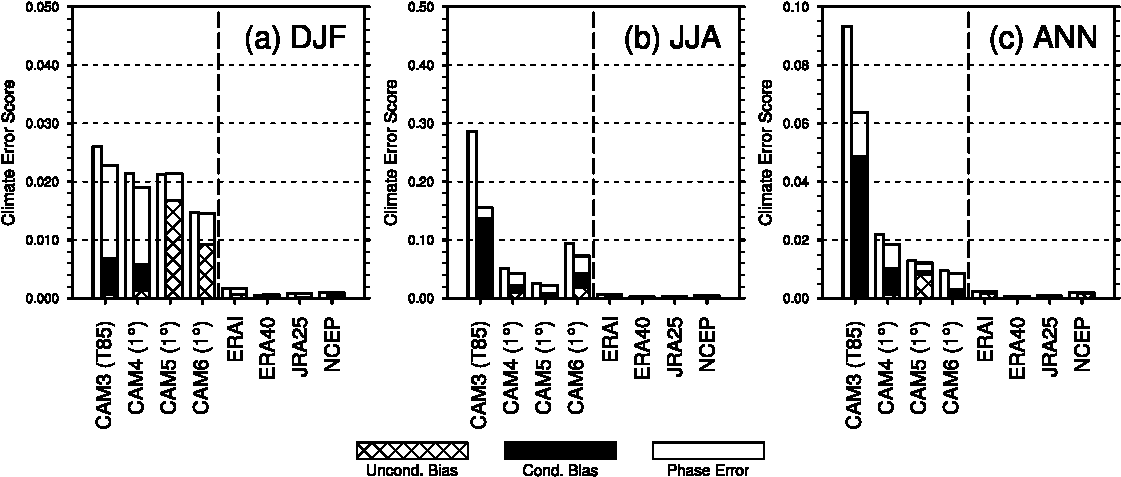
\includegraphics[width=1\textwidth,angle=0.]{./figs/f_skill_score.pdf}
 \end{center}
  \caption {Seasonal climatology of contributions to the Normalized Mean Square Error (NMSE) over the northern hemisphere (30$^\circ$ N-90$^\circ$ N) for CAM releases between CAM3 and CAM6. Individual contributions are the unconditional bias (hatched), conditional bias (solid) and phase error (unfilled). The narrow unfilled bar for each model is the scaled variance ratio (SVR). The model is compared to the ECMWF (ERA15) reanalysis. Contemporary analysis (JRA25/NCEP/ERA40 and ERA-interim) biases compared top ECMWF are also shown.} 
\label{f_skill_score}
\end{figure} 
%%
\clearpage
\begin{figure}[t]
  \begin{center}
    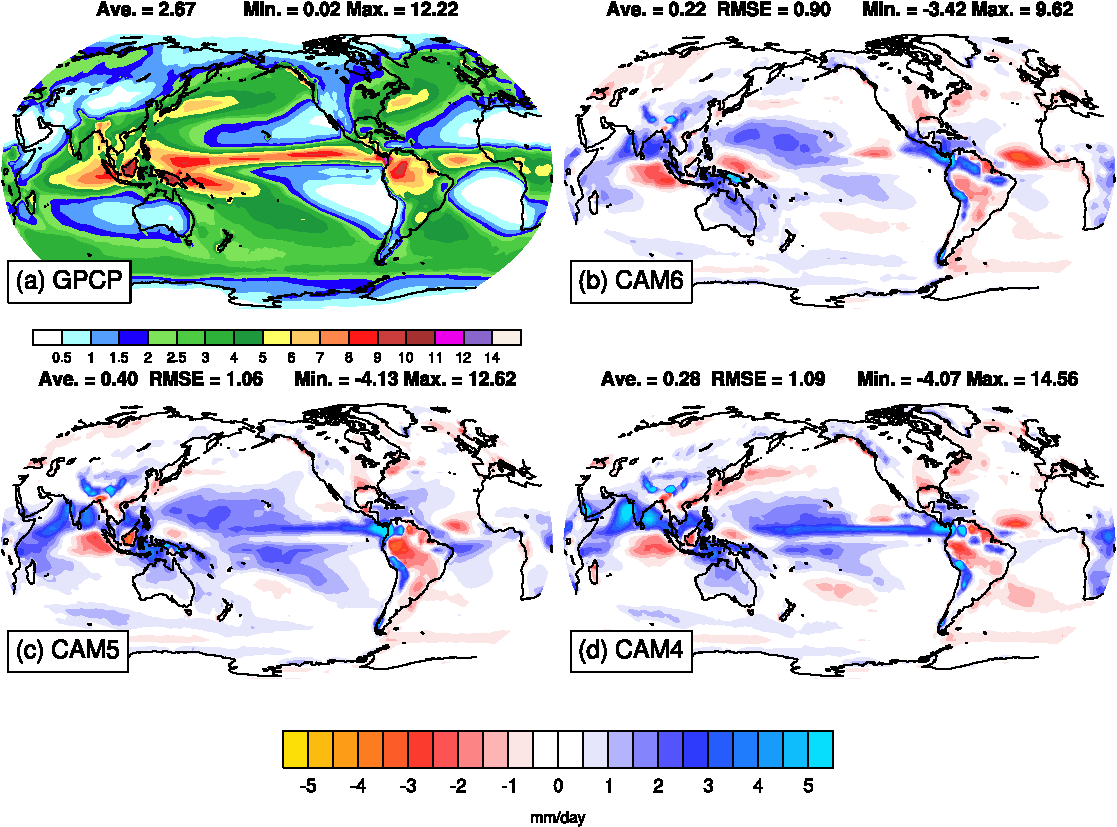
\includegraphics[width=1.\textwidth,angle=0.]{./figs/f_PRECT_2D_CAM456.pdf}
  \end{center}
  \caption{Climatology of annual precipitation (mm/day) for (a) Observations (GPCP, 19XX-20XX), and its biases for (a) CAM4 (b) CAM5  through CAM6 AMIP simulations for the period 1979-2005} 
\label{f_PRECT_2D_CAM456}
\end{figure} 
%%
\clearpage
\begin{figure}[t]
  \begin{center}
    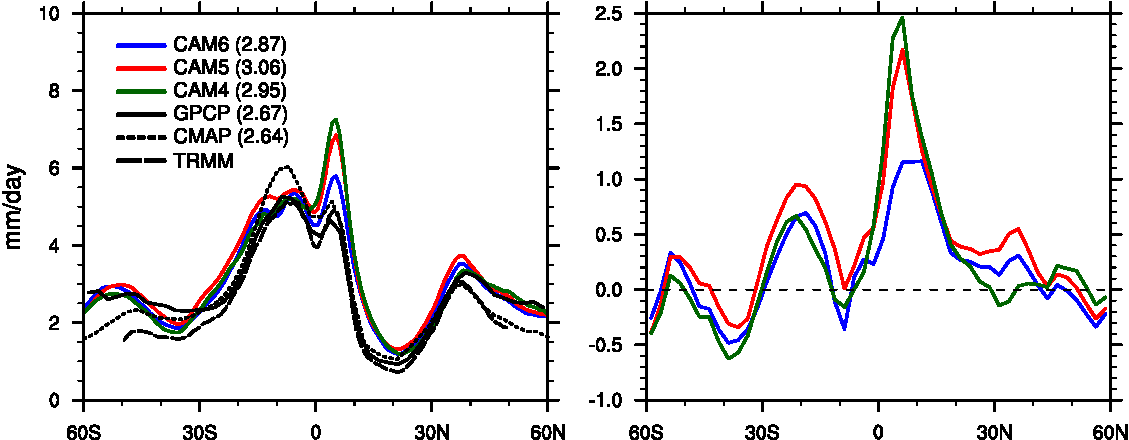
\includegraphics[width=1.\textwidth,angle=0.]{./figs/f_PRECT_1D_DJF_CAM456.pdf}
  \end{center}
  \caption{Climatology of annual precipitation (mm/day) for (a) Observations (GPCP, 19XX-20XX), and its biases for (a) CAM4 (b) CAM5  through CAM6 AMIP simulations for the period 1979-2005} 
\label{f_PRECT_1D_DJF_CAM456}
\end{figure} 
%%
\clearpage
\begin{figure}[t]
  \begin{center}
    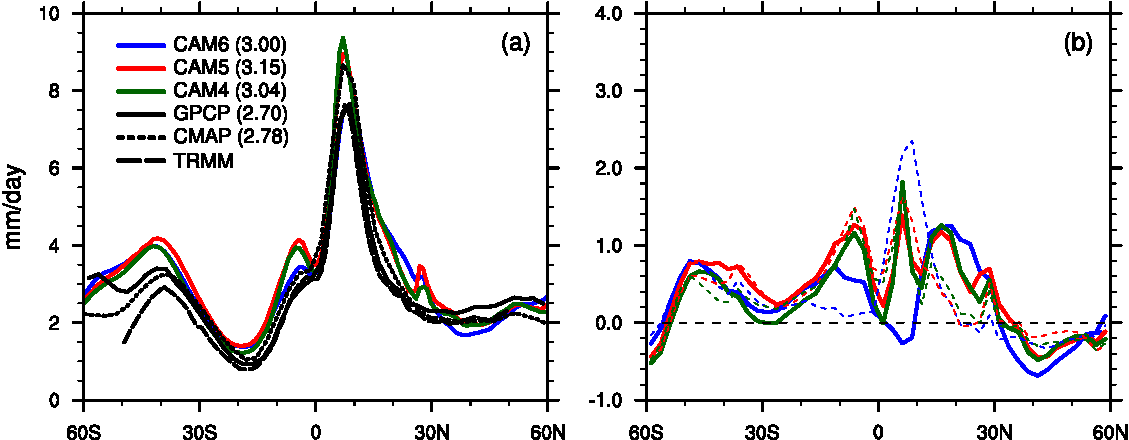
\includegraphics[width=1.\textwidth,angle=0.]{./figs/f_PRECT_1D_JJA_CAM456.pdf}
  \end{center}
  \caption{Climatology of annual precipitation (mm/day) for (a) Observations (GPCP, 19XX-20XX), and its biases for (a) CAM4 (b) CAM5  through CAM6 AMIP simulations for the period 1979-2005} 
\label{f_PRECT_1D_JJA_CAM456}
\end{figure} 

%%
\clearpage
\begin{figure}[t]
  \begin{center}
    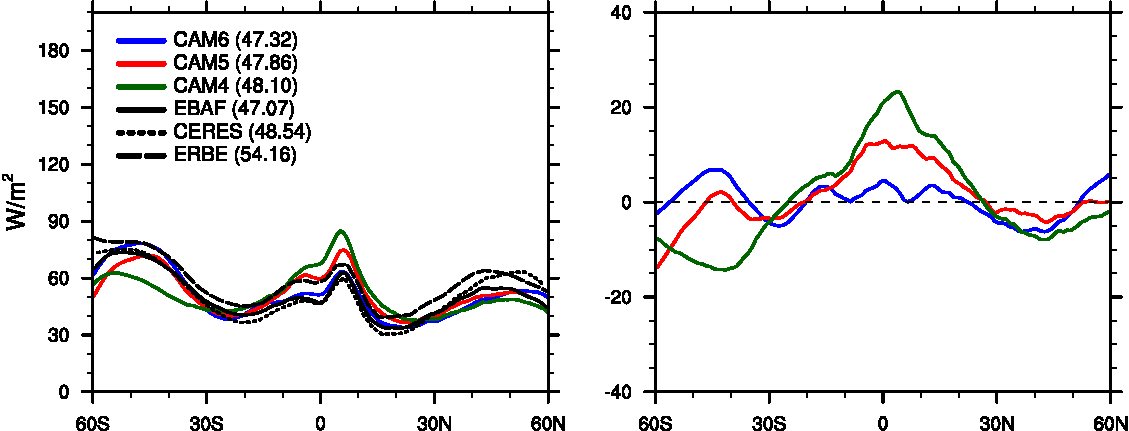
\includegraphics[width=1.\textwidth,angle=0.]{./figs/f_SWCF_1D_ANN_CAM456.pdf}
  \end{center}
  \caption{Climatology of annual precipitation (mm/day) for (a) Observations (GPCP, 19XX-20XX), and its biases for (a) CAM4 (b) CAM5  through CAM6 AMIP simulations for the period 1979-2005} 
\label{f_SWCF_1D_ANN_CAM456}
\end{figure} 

%%
\clearpage
\begin{figure}[t]
  \begin{center}
    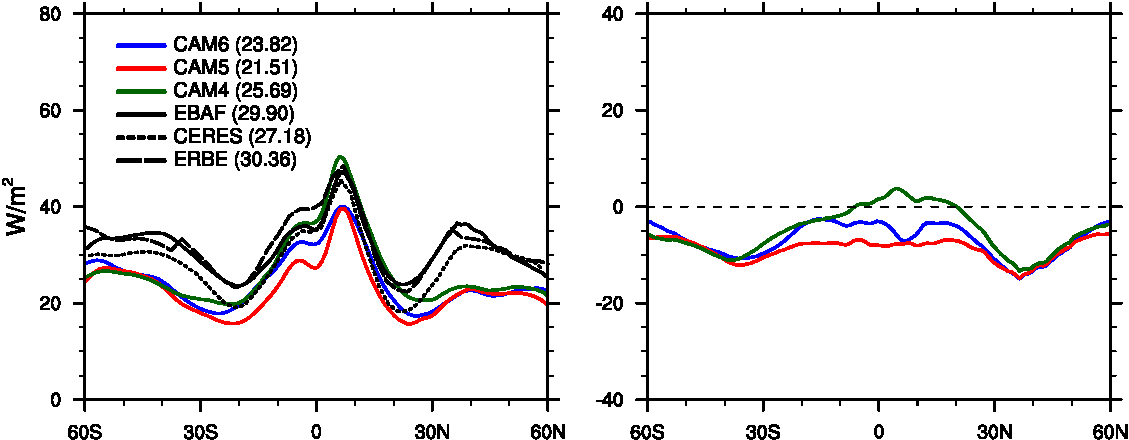
\includegraphics[width=1.\textwidth,angle=0.]{./figs/f_LWCF_1D_ANN_CAM456.pdf}
  \end{center}
  \caption{Climatology of annual precipitation (mm/day) for (a) Observations (GPCP, 19XX-20XX), and its biases for (a) CAM4 (b) CAM5  through CAM6 AMIP simulations for the period 1979-2005} 
\label{f_LWCF_1D_ANN_CAM456}
\end{figure} 

%%
\clearpage
\begin{figure}[t]
  \begin{center}
    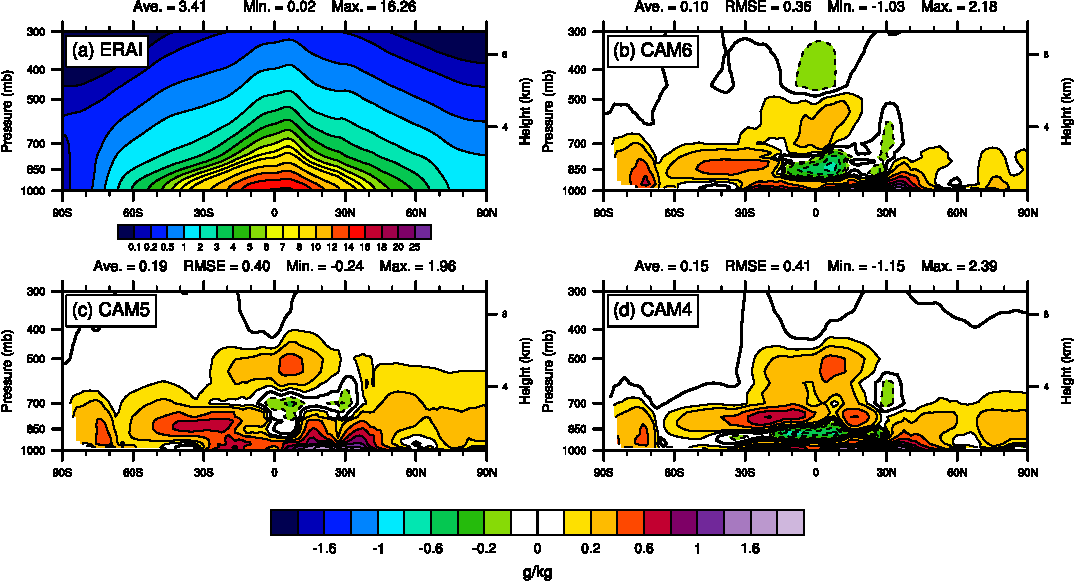
\includegraphics[width=1.\textwidth,angle=0.]{./figs/f_MERRA_Q_latp_diff_ANN.pdf}
  \end{center}
  \caption{Climatology of annual precipitation (mm/day) for (a) Observations (GPCP, 19XX-20XX), and its biases for (a) CAM4 (b) CAM5  through CAM6 AMIP simulations for the period 1979-2005} 
\label{MERRA_Q_latp_diff_ANN}
\end{figure} 



%% ------------------------------------------------------------------------ %%
%%  REFERENCE LIST AND TEXT CITATIONS
%


% For supplementary material like Cecile's table
%\input{supplementary.tex}



%  END ARTICLE
%

\end{document}


%%%%%%%%%%%% MOVE ALL INFORMATIONAL TEXT JIC its needed %%%%%%%%%%%%%%


% 
%% ------------------------------------------------------------------------ %%
%
%  SIDEWAYS FIGURE AND TABLE EXAMPLES
%
%% ------------------------------------------------------------------------ %%
%
% For tables and figures, add \usepackage{rotating} to the paper and add the rotating.sty file to the folder.
% AGU prefers the use of {sidewaystable} over {landscapetable} as it causes fewer problems.
%
% \begin{sidewaysfigure}
% \includegraphics[width=20pc]{samplefigure.eps}
% \caption{caption here}
% \label{label_here}
% \end{sidewaysfigure}
%
%
%
% \begin{sidewaystable}
% \caption{}
% \begin{tabular}
% Table layout here.
% \end{tabular}
% \end{sidewaystable}
%
%
%%%%%%%%%%%%%%%%%%%%%%%%%%%%%%%%%%%%%%%%%%%%%%%%%%%%%%%%%%%%%%%%%%%%%%%%%
% Figures and Tables
%
%
% DO NOT USE \psfrag or \subfigure commands.
%
%  Figures and tables should be placed AT THE END OF THE ARTICLE,
%  after the references.
%
%  Uncomment the following command to include .eps files
%  (comment out this line for draft format):
%  \usepackage[dvips]{graphicx}
%
%  Uncomment the following command to allow illustrations to print
%   when using Draft:
%  \setkeys{Gin}{draft=false}
%
% Substitute one of the following for [dvips] above
% if you are using a different driver program and want to
% proof your illustrations on your machine:
%
% [xdvi], [dvipdf], [dvipsone], [dviwindo], [emtex], [dviwin],
% [pctexps],  [pctexwin],  [pctexhp],  [pctex32], [truetex], [tcidvi],
% [oztex], [textures]
%
% See how to enter figures and tables at the end of the article, after
% references.
%
%% ------------------------------------------------------------------------ %%
%
%  ENTER PREAMBLE
%
%% ------------------------------------------------------------------------ %%
% To create numbered lines:

% If you don't already have lineno.sty, you can download it from
% http://www.ctan.org/tex-archive/macros/latex/contrib/ednotes/
% (or search the internet for lineno.sty ctan), available at TeX Archive Network (CTAN).
% Take care that you always use the latest version.

% To activate the commands, uncomment \usepackage{lineno}
% and \linenumbers*[1]command, below:

% \usepackage{lineno}
% \linenumbers*[1]

%  To add line numbers to lines with equations:
%  \begin{linenomath*}
%  \begin{equation}
%  \end{equation}
%  \end{linenomath*}


% Author names in capital letters:
%\authorrunninghead{Neale et al. 2019}

% Shorter version of title entered in capital letters:
%\titlerunninghead{CAM6 Overview}

%Corresponding author mailing address and e-mail address:
%\authoraddr{Corresponding author: A. B. Smith,
%Department of Hydrology and Water Resources, University of
%Arizona, Harshbarger Building 11, Tucson, AZ 85721, USA.
%(a.b.smith@hwr.arizona.edu)}